\documentclass[12pt, letterpaper]{report}
\usepackage[newfloat]{minted}
\usepackage{caption}
\usepackage{tocloft}
\usepackage{acro}
\usepackage{pdfpages}
\usepackage[toc,page,title]{appendix}
\usepackage[colorlinks=true]{hyperref}
\usepackage{graphicx}
\definecolor{usfgreen}{rgb}{0, 0.40, 0.28}
\newcommand*{\sectref}[1]{\hypersetup{linkcolor=usfgreen}\hyperref[{#1}]{\ref*{#1}: \nameref*{#1}}}
\newcommand*{\itemref}[1]{\hypersetup{linkcolor=usfgreen}\hyperref[{#1}]{\autoref*{#1}: \nameref*{#1}}}
\newcommand*{\boxedimage}[1]{\fbox{\includegraphics[width=0.5\textwidth]{#1}}}
\newcommand{\fig}[3]{
  \begin{figure}[h]
    \caption{#1}
    \label{#3}
    \centering
    \boxedimage{#2}
  \end{figure}
}
\newcommand*{\descitem}[1]{\item[#1] \hfill \\ }

% class `abbrev': abbreviations:
\DeclareAcronym{omr}{
  short = OMR ,
  long  = Optical mark recognition ,
  class = abbrev
}
\DeclareAcronym{oer}{
  short = OER ,
  long  = Open educational resources ,
  class = abbrev
}
\DeclareAcronym{csv}{
  short = CSV ,
  long  = Comma seperated values [file] ,
  class = abbrev
}

\begin{document}
\definecolor{bg}{rgb}{0.95,0.95,0.95}
\frenchspacing
\newenvironment{ex}{\captionsetup{type=listing}}{}
\SetupFloatingEnvironment{listing}{name=Code Sample}
\newcommand{\listcodesamples}{List of Code Samples}
\newlistof{codesample}{mcf}{\listcodesamples}

\newcommand{\codesample}[1]
{
    \captionof{listing}{#1}
    \refstepcounter{codesample}
    \addcontentsline{mcf}{codesample}
    {\protect\numberline{\thecodesample}#1}\par
}

\hyphenation{pro-hib-it-ive-ly Scan-tron ubiq-uit-ous cor-respond-ing Auto-matic}

\acsetup{first-style=short}

\AtBeginEnvironment{appendices}{\renewcommand\thesection{Appendix~\Alph{section}}}
\renewcommand{\appendixname}{Appendix}

\title{Test Latex Doc}
\author{Ian Sanders}
\date{December 2019}
\maketitle

\begin{abstract}
Lorem ipsum `dolor' sit amet.
\end{abstract}

\tableofcontents
\listofcodesample
\printacronyms[include-classes=abbrev,name=Abbreviations]

\chapter{Introduction}
\section{Background}
Optical mark recognition (\ac{omr}) is a ubiquitous technology whenever large amounts
of controlled physical data needs to be converted to a digital form. This is an
especially common task in the field of education, where the scoring of dozens to
hundreds of multiple choice tests is a regular need. Manual grading of such
examinations is a mundane and time-consuming task that can be easily avoided
with the use of \ac{omr}, as the submission format is completely controlled.
\section{Existing Solutions}
Many of the most popular \ac{omr} solutions presently available are prohibitively
expensive. The most popular product available, sold by Scantron, consists of a
proprietary scanner that is only compatible with Scantron sheets. The scanner
alone can cost several thousand dollars, and the sheets present a continuing
cost for as long as the scanner is in use.

An increasing interest in open educational resources (\ac{oer}) has led to the
development of several free and open source solutions, such as: FormScanner,
queXF, and Auto Multiple Choice. These softwares work extremely well, however,
they have failed to become mainstream due to their increased complexity. Thus,
there exists a need for a simple, free solution that can be implemented with
minimal training or setup time.
\section{Proposed Solution}
A simple, freely available software and mark sheet pair is proposed. By
providing a freely available mark sheet in printable form, setup time is reduced
to the time it takes to download and print the file. In addition, a simple,
easy-to-use software utility that prioritizes reliability will encourage
educators to make the transition from proprietary solutions to an open and free
one. The software will remain simple while still providing a competitive feature
suite and will act as a bridge between raw exam results and more full-featured
exam analysis software.
\subsection{Requirements}
Based on the problem analysis and proposed solution, the final product should:

\begin{enumerate}
  \item Be freely available and open-source
  \item Be as reliable as possible in order to produce fair results
  \item Process files in bulk
  \item Be simple and easy to learn and use
  \item Sort results
  \item Output files that can be input into analysis software
  \item Require minimal setup
  \item Be immediately understood by students taking exams
  \item Provide readily available training resources for educators
  \item Complete processing of results in reasonable amount of time
\end{enumerate}


\chapter{Design of Multiple Choice Sheet}
The multiple-choice sheet is the physical piece of paper that all students
taking exams will fill out. It is also known as a `bubble sheet', easily recognized
by many due to its grid of circles that must be filled in to input answers. In order to
develop a reliable solution with minimal setup, only one sheet is supported
by the software. Therefore, this sheet must be highly optimized.

In order to ensure that the entire solution is freely available to all
educators, an entirely new multiple-choice sheet was developed for use.
This new sheet balances optimization for optical mark recognition with
user-friendliness.

\section{Design Overview}
The optical mark sheet designed for this project consists of several sections,
or `fields'. Several fields provide empty boxes for students to write in their
answers. This provides the administrator with a means to rapidly identify tests
and verify student information. The data fields
also have banded columns to aid users in easily filling in data despite the
larger grids. The completed design is shown in
\itemref{fig:sheet}, while a full printable version is given in \sectref{sect:sheet}.

\fig{Final multiple-choice sheet design.}{sheet.png}{fig:sheet}

The sheet consists of a `student information' section and an `answers' section,
divided by a location for student signatures. The following fields are
included:
\begin{description}
  \descitem{Last Name} For the student's last name. Space for 12 alphabetic
  characters is provided.
  \descitem{First [Name]} For the student's first name. Space for 6 alphabetic
  characters is provided.
  \descitem{Middle [Name]} For the student's middle name. Space for 2 alphabetic
  characters is provided\footnote{It is expected that any students who have a
  middle name will likely have a middle name longer than two characters; this
  is considered acceptable as the middle name is used primarily for sorting.}.
  \descitem{Student ID} For any ID number that identifies students. This could be an
  official institutional ID or simply a number given by the administrator. Space
  for 10 numeric digits is given.
  \descitem{Course ID} For an ID number that identifies the course. Again, this
  could be official per the institution, or a number generated by the
  administrator to identify the course and section. Space for 10 numeric digits
  is given.
  \descitem{Test Form Code} The optional test form code matches exam results with
  their corresponding answer keys. As described in \sectref{sect:scoring}, this can
  be a single character or multiple.
  \descitem{Signature} An informal (unprocessed) field is provided for the exam-
  taker's signature. This does not affect results in any way.
  \descitem{Date} An informal (unprocessed) field is provided for the date. This is
  intended to pair with the Signature field and thus does not affect results
  either.
  \descitem{Answers} The core of the multiple-choice sheet is the set of up to 75
  multiple-choice answers to fill in. The test designer can choose to use
  anywhere from 1 to 75 questions, with answers A-F (or any combination of 2 or
  more of those), as described in \sectref{sect:scoring}.
\end{description}


\section{Features}
Two primary features make the multiple-choice sheet optimal for use with \ac{omr}.

\subsection{Grid System}
In order to ease the mark recognition process, everything on the sheet is aligned
to a grid of $^3/_{16}"$ squares, as can be seen in \itemref{fig:grid}. This
enables the rapid identification of optical marks without the need for complex
and inconsistent shape-finding algorithms, as described in
\sectref{sect:process}. Not only are items aligned to a grid within their own
field, but also on the same grid as every other item on the sheet
\fig{Multiple-choice sheet with grid visible.}{grid.png}{fig:grid}

\subsection{Corner Marks}
A reliable means for establishing the corners of the grid is essential for
reading any data. To this end, an easily-recognized `corner mark' is provided,
with the far corners of each matching perfectly with the grid corners (as shown
in \itemref{fig:corners}). The corner detection process is described in detail
in \sectref{sect:cornerfinding}, but in short, the algorithm first seeks the
\textbf{L}-shaped mark in the top left corner, and then looks for squares of the
expected size and in the expected location to identify the other marks.

As all marks are constructed from
squares of the same size, the expected size of the other three marks can easily
be obtained. Thus, filtering out other square shapes (such as the write-in field
boxes) is simple as they are a different size.

The marks are intentionally dark enough that they will be easily located when
processed with nearly any printer/scanner combination, but they are only 60\%
gray in order to avoid becoming a distraction for exam-takers. Not only could
distractions negatively impact exam scores; they could also attract unwanted
attention that might result in idle doodling or defacing and render
mark recognition impossible.
\fig{Detail view of multiple-choice sheet corner marks.}{corner_marks.png}{fig:corners}

\chapter{Design of \ac{omr} Software}
The software developed to read the multiple-choice sheets is a free, open-source
utility called \textit{OpenMCR}. This tool provides a simple interface to the
complex process of importing, preprocessing, and reading the filled sheets.
\fig{Logo for OpenMCR software utility.}{logo.png}{fig:logo}

\section{User Interface Design}
OpenMCR provides test administrators with a simple, intuitive interface in which
every option is available on a single screen (\itemref{fig:mainscreen}). Use of the software follows a
simple process from the top of the screen to the bottom:
\begin{enumerate}
  \item The user selects a folder to import image files from. All image files
  located directly in the selected folder will be used.
  \item The user chooses, through simple checkboxes, whether or not to convert
  empty answers to the letter \textbf{G} and multiple selected answers to the
  letter \textbf{F}. This can aid with postprocessing of results.
  \item [Optional] The user can upload a custom \ac{csv} file to use as an
  answer key. As described in \sectref{sect:scoring}, the user can also create
  keys using the multiple-choice files themselves, or choose not to provide any
  keys at all.
  \item [Optional] The user can upload a rearrangement \ac{csv} file for
  reordering results based on keys. This can aid with postprocessing of results
  as described in \sectref{sect:rearranging}.
  \item The user selects an output folder to save results in.
  \item The user can choose whether or not to sort results --- again by toggling
  a simple checkbox.
\end{enumerate}
\fig{Main input screen of OpenMCR.}{main_screen.png}{fig:mainscreen}

At the bottom of the screen, a \textit{status} section is provided (\itemref{fig:statuses}). Whenever the
user makes a choice or completes a step, the status messages are updated. When
all error messages are resolved (ie, all required steps are completed), the
\textbf{Continue} button is enabled and processing can be started.

\fig{Examples of potential status messages.}{statuses.png}{fig:statuses}

Two additional buttons are also provided:
\begin{description}
  \descitem{Open Sheet} Opens the multiple-choice sheet PDF directly, making it
  simple and easy to print out more sheets.
  \descitem{Open Help} Opens a PDF file with the entire user manual for the
  software, ideally resolving all problems rapidly and efficiently.
\end{description}

When the user presses \textbf{Continue}, a progress bar appears and any error
messages are shown in the status. Upon completion, a success message and \textbf{Close}
button are shown. These are visible in \itemref{fig:progress}.

\fig{OpenMCR status section during (top) and after (bottom) processing.}{progress.png}{fig:progress}


\subsection{Features}
\subsubsection{Automatic Scoring}
\label{sect:scoring}
\subsubsection{Rearrangement by Key}
\label{sect:rearranging}
\subsubsection{Sorting Results}
\subsubsection{Output Files}
\section{Optical Mark Recognition Process}
\label{sect:process}
\subsection{Image Preprocessing}
\subsection{Corner Detection}
\label{sect:cornerfinding}
\subsection{Grid Establishment}
\subsection{Mark Reading}
\begin{appendices}
\section{Acknowledgements}
\section{Licenses}
\label{sect:licenses}
\section{Multiple-Choice Sheet}
\label{sect:sheet}
The full printable multiple-choice sheet is available on the next page. See
\sectref{sect:licenses} for the license information for this sheet.
%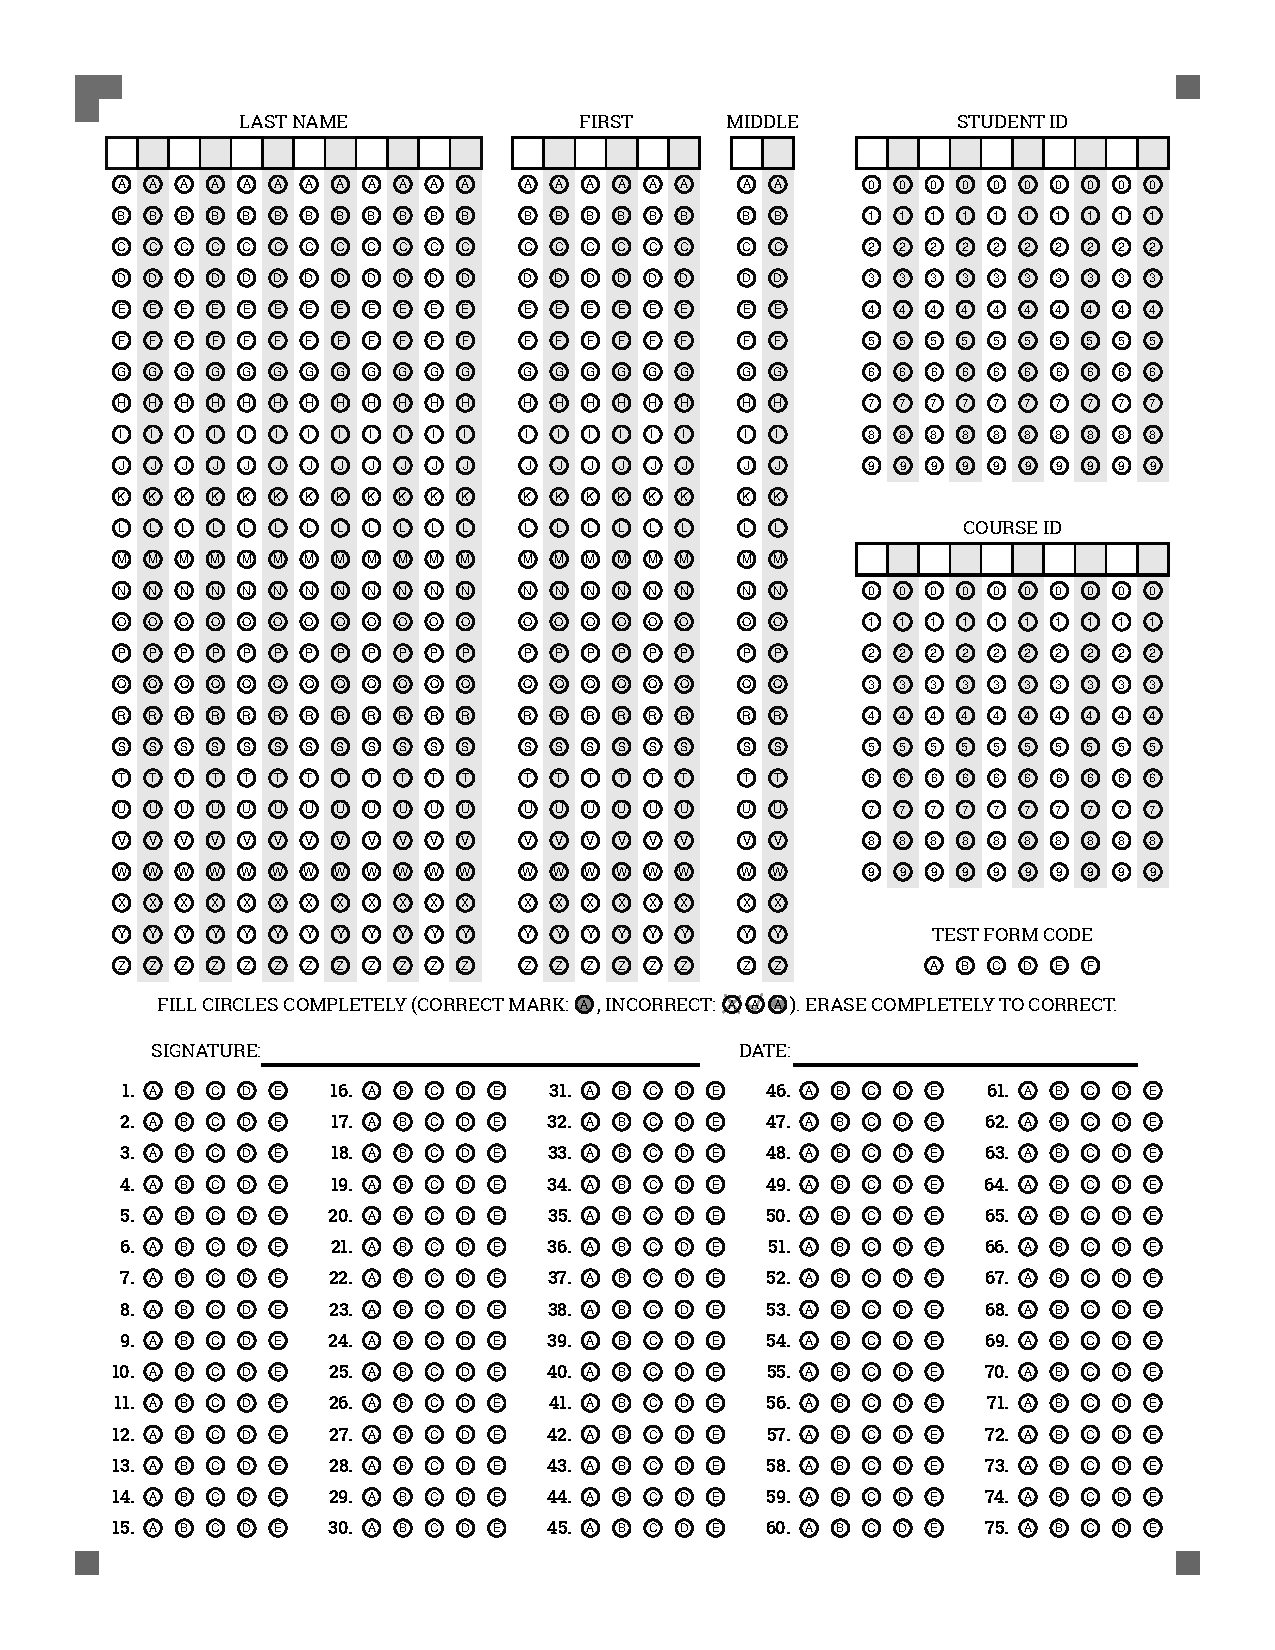
\includepdf{sheet.pdf} 
\end{appendices}
\end{document}